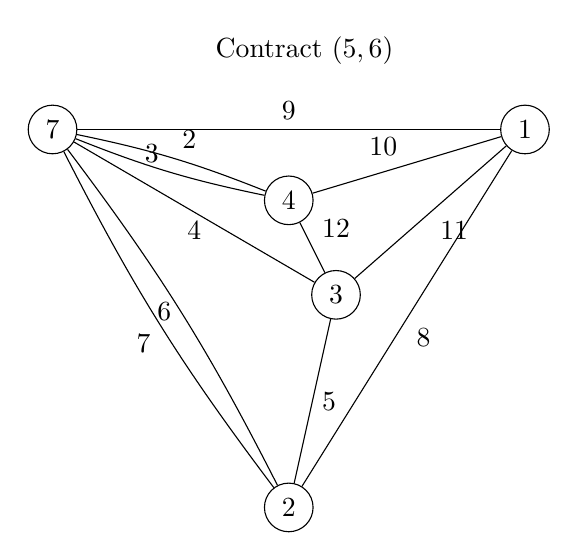
\begin{tikzpicture}
	\node (G) at (2, 1) {Contract $(5,6)$};
	% Define the nodes with specific positions
	\begin{scope}[xshift=0cm, yshift=0cm, scale=0.6]
		\node[circle, draw] (1) at (8, -0) {1};
		\node[circle, draw] (2) at (3, -8) {2};
		\node[circle, draw] (3) at (4, -3.5) {3};
		\node[circle, draw] (4) at (3, -1.5) {4};
		\node[circle, draw] (7) at (-2, -0) {7};
	
		% Draw the edges between nodes with labels
		\draw[draw] (7) to[bend left=5] node[above right] {2} (4);
		\draw[draw] (4) to[bend left=5] node[above left] {3} (7);
		\draw[draw] (3) -- node[below] {4} (7);
		\draw[draw] (3) -- node[right] {5} (2);
		\draw[draw] (7) to[bend left=5] node[left] {6} (2);
		\draw[draw] (2) to[bend left=5] node[below left] {7} (7);
		\draw[draw] (1) -- node[below right] {8} (2);
		\draw[draw] (1) -- node[above] {9} (7);
		\draw[draw] (1) -- node[above left] {10} (4);
		\draw[draw] (1) -- node[below right] {11} (3);
		\draw[draw] (4) -- node[above right] {12} (3);
	\end{scope}
\end{tikzpicture}